
In an effort to provide a solution to the interoperability problem, the Object 
Management Group (OMG) created the Common Object Request Broker Architecture
(CORBA).  \cite{siegel}  CORBA is OMG's open, vendor-independent architecture 
and infrastructure that computer applications use to work together over networks.
\cite{omg} By using the Internet Inter ORB Protocol (IIOP), a CORBA-based program 
from any vendor, on almost any computer, operating system, programming language, 
and network, can inter-operate with a CORBA-based program from the same or another 
vendor, on almost any other computer, operating system, programming language, 
and network. \cite{omg} Since CORBA is based upon object orientation, you must 
define each CORBA object's interface in OMG's Interface Definition Language (IDL). 
This fixes the operations the CORBA object will perform, and the input and output 
parameters each will accept.\cite{siegel} This interface definition is independent 
of your programming language. \cite{omg} The interface to each CORBA object is 
defined very strictly. But, in contrast, the implementation of a CORBA object
is hidden from the rest of the system behind a boundary that the client may not 
cross. Clients access CORBA objects only through their advertised interface, 
invoking only those operations that the object chooses to expose, with only 
those parameters that are included in the invocation. \cite{omg}

In order to create a CORBA-based application, you must compile the IDL 
specification for the objects you wish to utilize.  This compilation will 
generate IDL stubs and skeletons for the objects defined within the IDL
specification.  Once the stubs and skeletons have been generated, the 
object can be implemented and a client application can be written to 
utilize the functionality of the object.  
These IDL stubs and skeletons act as proxies for the client application and 
object implementation.\cite{omg} 
Figure \ref{RequestPassing} illustrates the use of IDL stubs and skeletons as 
a client application's request is being passed to a CORBA object.  
 
\begin{figure}
\begin{center}
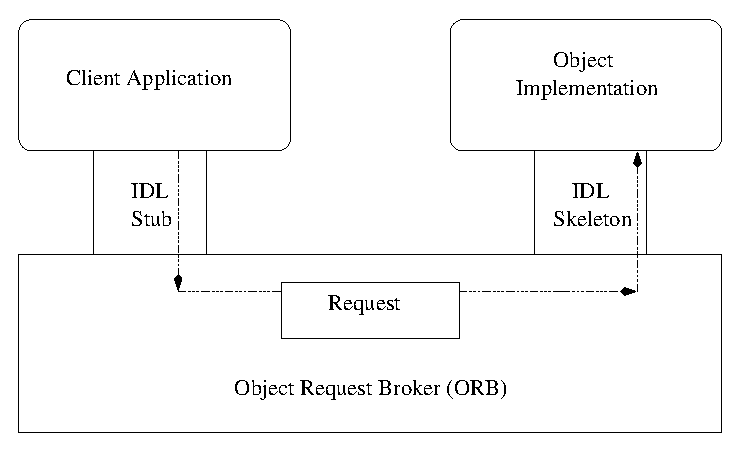
\psfig{file=Figures/RequestPassing.eps}
\leavevmode
\caption{\em{A request passing from a client application to an object implementation using the same ORB}.}
\figline
         \label{RequestPassing}
\end{center}
\end{figure}

When CORBA is being used to communicate between objects that reside 
on the same computer, the scenario depicted in figure \ref{RequestPassing}
could accurately illustrate the necessary path of communication for an 
invocation request.  However, when objects reside on remote computers, 
communication must take place between multiple ORBs.  The scenario where a 
client invokes an operation on a remote CORBA object is illustrated in 
figure \ref{ORB2ORB}.   
Since the standard Internet Inter ORB Protocol is being used to communicate 
between the ORBs, the ORBs can be from different vendors and still inter-operate
with ease.   
For more information on CORBA, the author recommends {\em{CORBA 3: Fundamentals
and Programming}} by Jon Siegel, PhD.  
\begin{figure}
\begin{center}
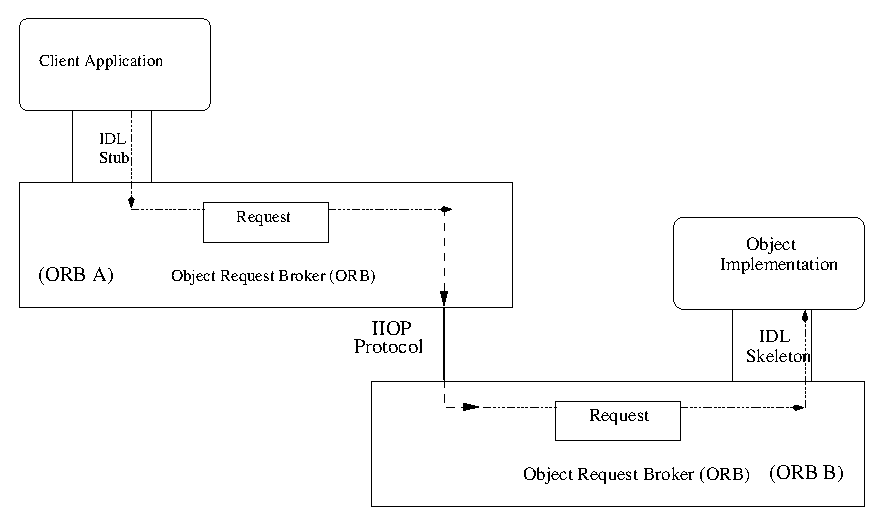
\psfig{file=Figures/ORB2ORB.eps}
\leavevmode
\caption{\em{A request passing from a client application using ORB A to an object implementation using ORB B}.}
\figline
         \label{ORB2ORB}
\end{center}
\end{figure}
